\chapter{Resultados}
Neste capítulo serão descritos os resultados obtidos através da simulação da
EDP com a variação de diversos parâmetros. Os parâmetros iniciais escolhidos
para este trabalho foram:
\begin{itemize}
    \item $L_x = 20$m (comprimento do domínio)
    \item $nx = 400$ (número de células)
    \item $\bar{u} = 1$m/s (velocidade de escoamento)
    \item $t_\text{final} = 2$s  (tempo final de simulação)
    \item $\Delta x = \frac{L_x}{nx} = 0,05$m (passo no espaço)
    \item $\Delta t = 0,8\left( \frac{\Delta_x}{\bar{u}} \right) = 0,04$s
          (passo de tempo)
    \item $A = 100$
    \item $B = 1,5$
    \item $C = 4,0$
    \item $D = 6,0$
    \item $E = 2,0$
\end{itemize}

\section{Resultados para variações de $nx$}
Com a variação de $nx$, obtiveram-se os seguintes resultados:
\begin{figure}[H]
    \centering
    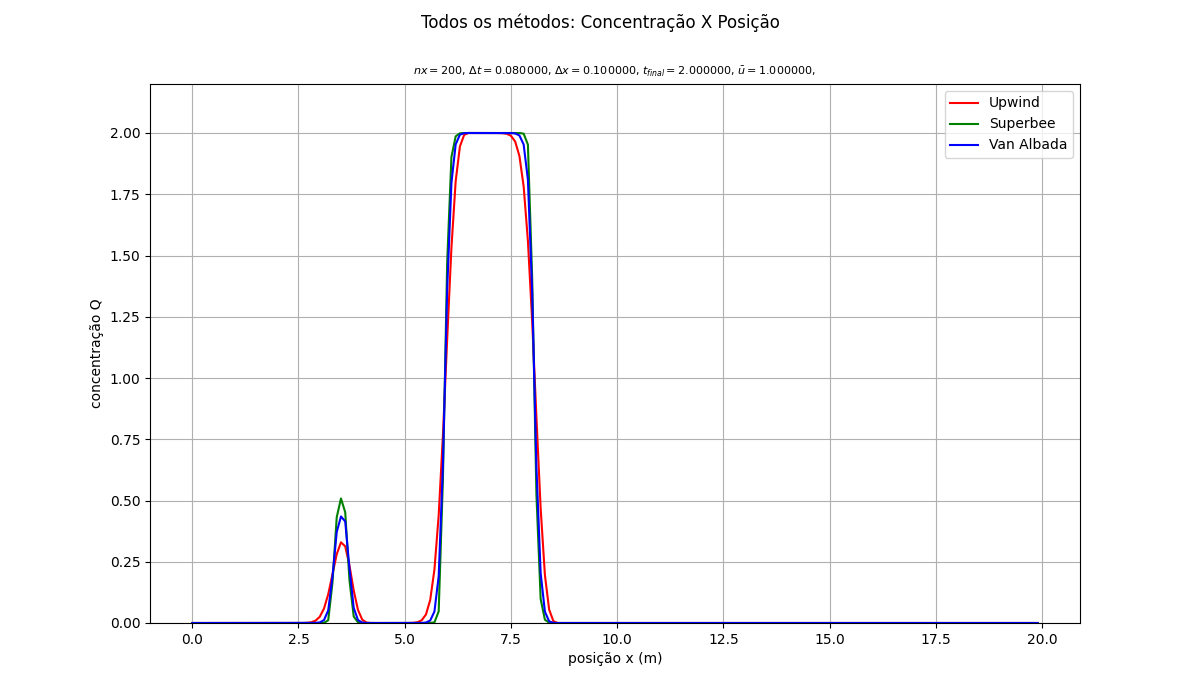
\includegraphics[width=0.7\textwidth]{methods_nx=200}
    \caption{FTBS, Superbee, Van Albada: $nx = 200$}
\end{figure}
\begin{figure}[H]
    \centering
    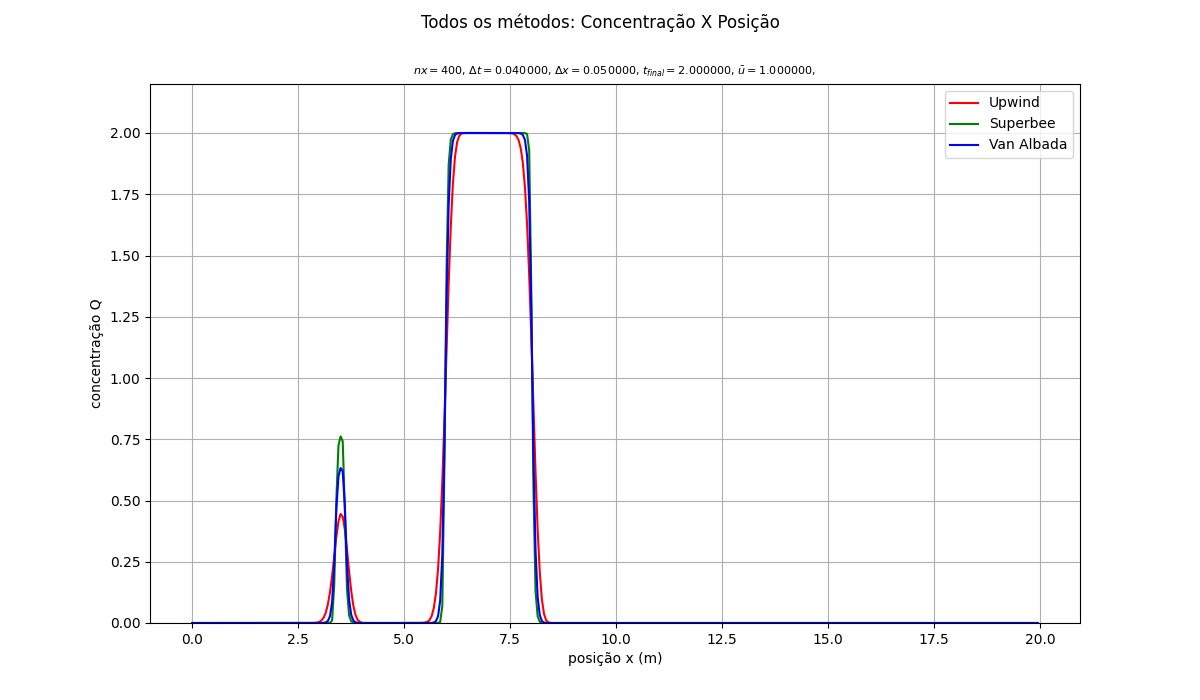
\includegraphics[width=0.7\textwidth]{methods_nx=400}
    \caption{FTBS, Superbee, Van Albada: $nx = 400$}
\end{figure}
\begin{figure}[H]
    \centering
    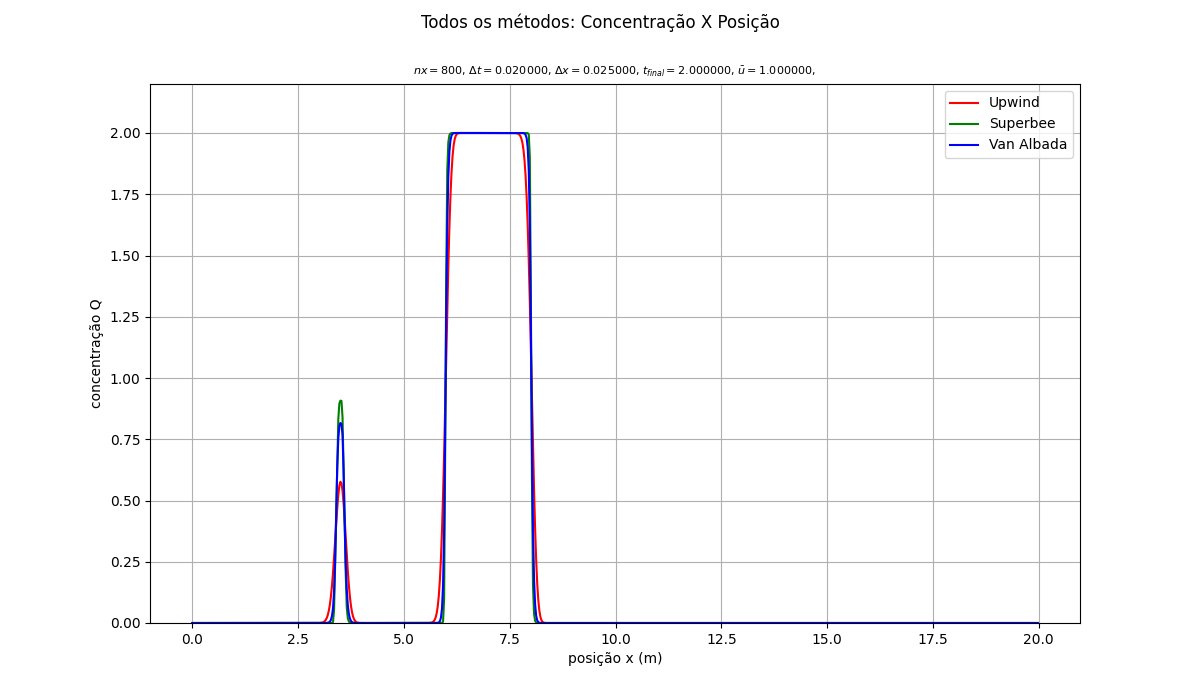
\includegraphics[width=0.7\textwidth]{methods_nx=800}
    \caption{FTBS, Superbee, Van Albada: $nx = 800$}
\end{figure}
\begin{figure}[H]
    \centering
    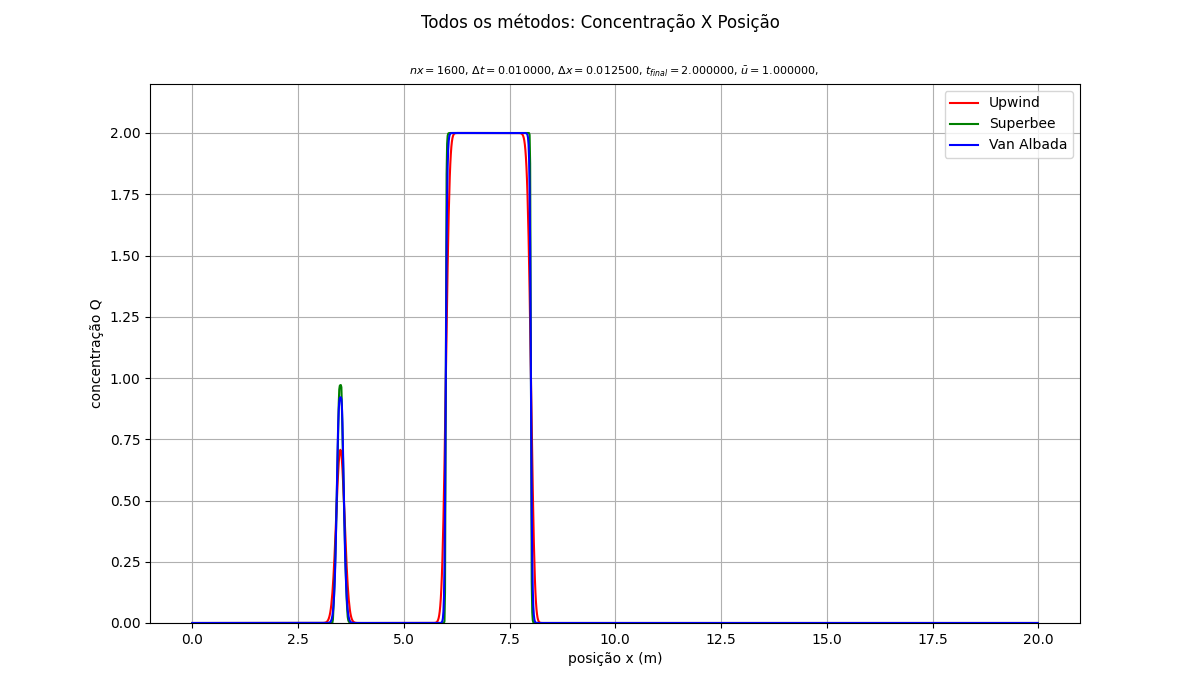
\includegraphics[width=0.7\textwidth]{methods_nx=1600}
    \caption{FTBS, Superbee, Van Albada: $nx = 1600$}
\end{figure}
Nota-se que o refinamento da malha resulta em dois fenômenos: a primeira onda
se torna mais ``pontiaguda'' e a segunda mais ``quadrada''; tais
características não podiam ser representadas em uma malha de baixa resolução.
Sendo assim, determina-se que o aumento no número de nós torna a solução
discreta mais próxima da analítica (solução real).

\section{Resultados para variações de $t_{\text{final}}$}
Com a variação de $t_{\text{final}}$, obtiveram-se os seguintes resultados:
\begin{figure}[H]
    \centering
    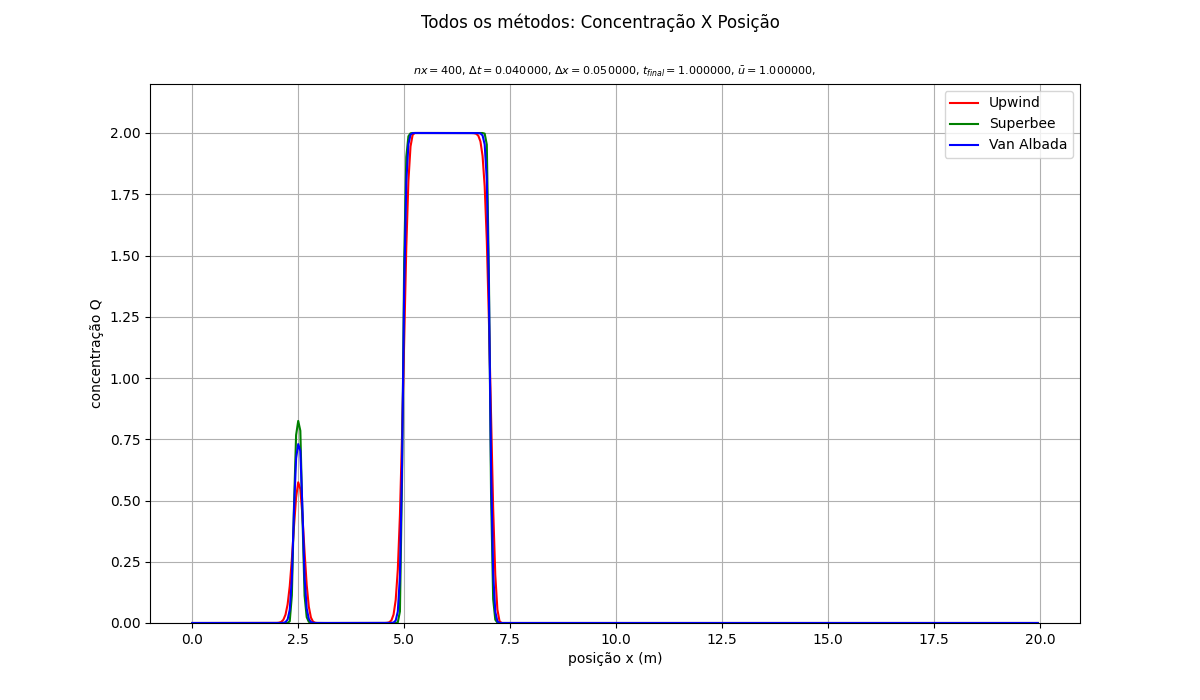
\includegraphics[width=0.7\textwidth]{methods_t=1.000000}
    \caption{FTBS, Superbee, Van Albada: $t_{\text{final}} = 1$s}
\end{figure}
\begin{figure}[H]
    \centering
    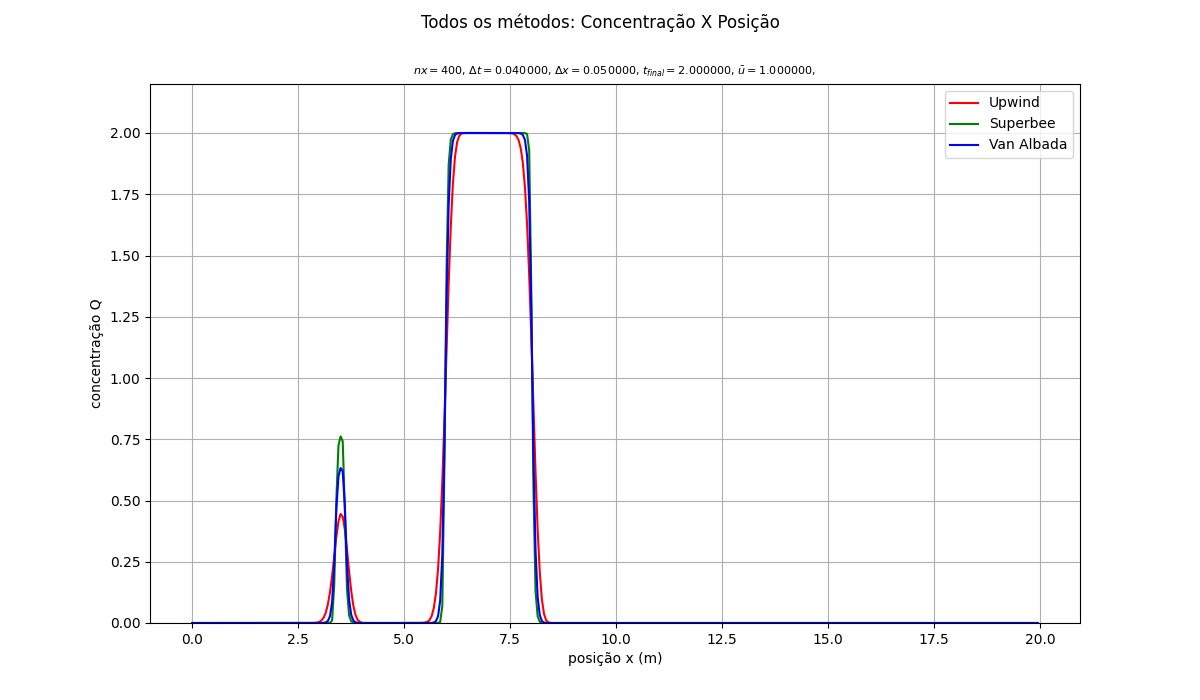
\includegraphics[width=0.7\textwidth]{methods_t=2.000000}
    \caption{FTBS, Superbee, Van Albada: $t_{\text{final}} = 2$s}
\end{figure}
\begin{figure}[H]
    \centering
    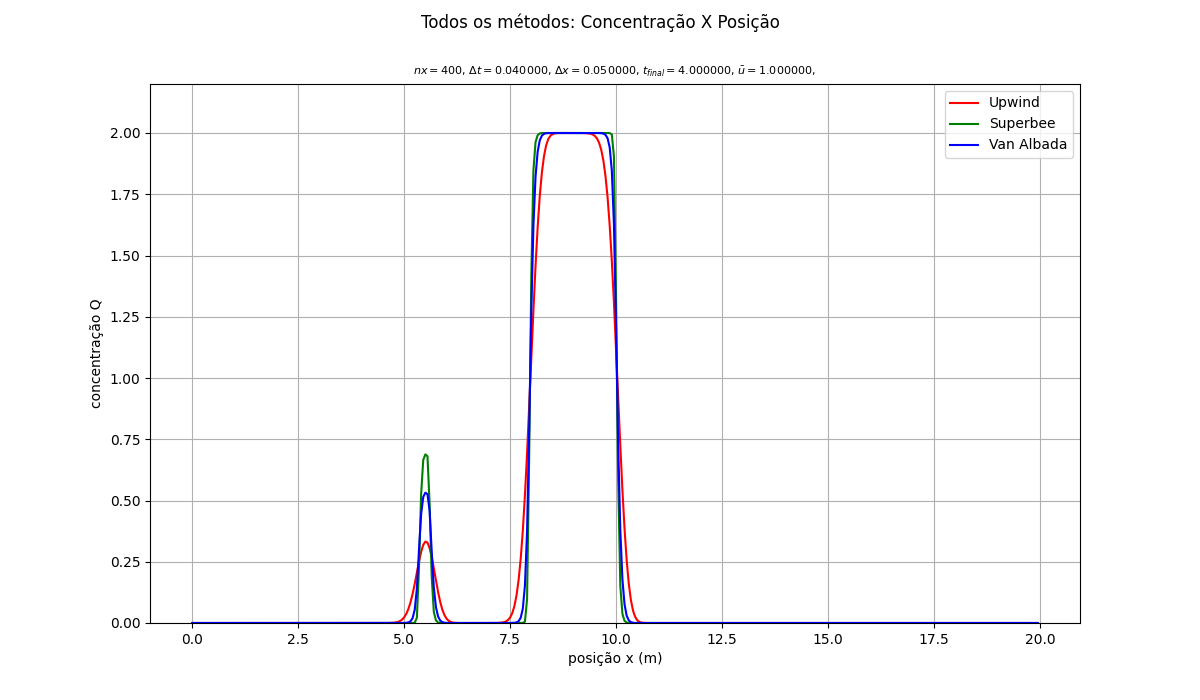
\includegraphics[width=0.7\textwidth]{methods_t=4.000000}
    \caption{FTBS, Superbee, Van Albada: $t_{\text{final}} = 4$s}
\end{figure}
\begin{figure}[H]
    \centering
    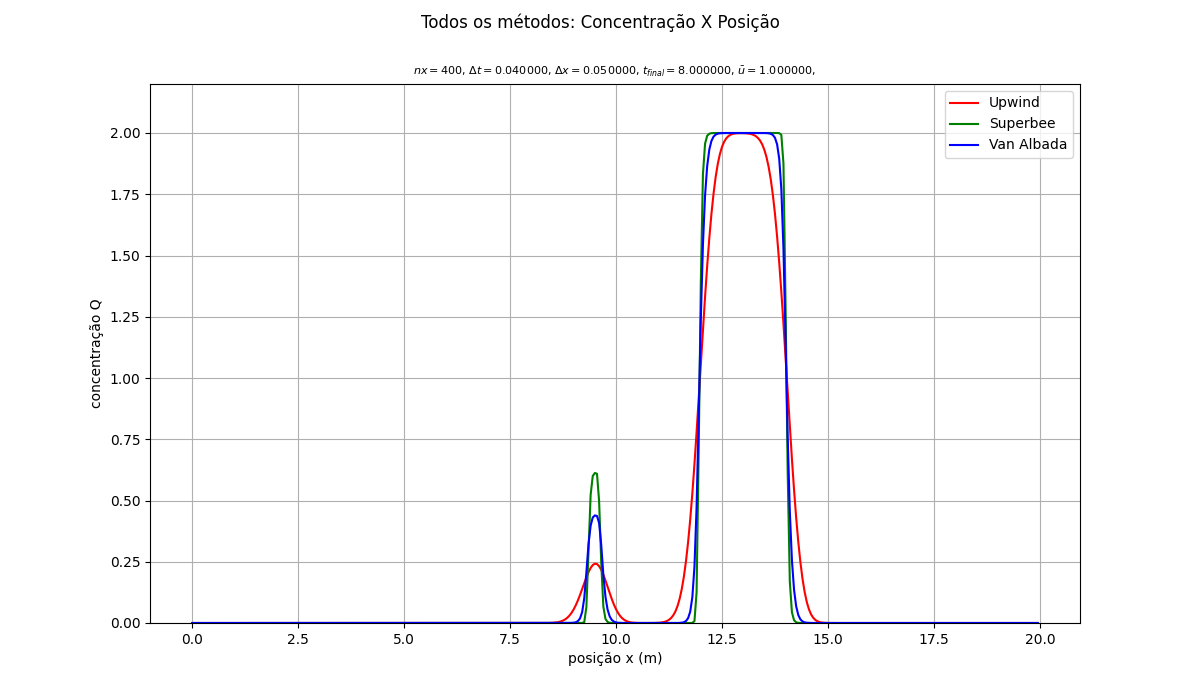
\includegraphics[width=0.7\textwidth]{methods_t=8.000000}
    \caption{FTBS, Superbee, Van Albada: $t_{\text{final}} = 8$s}
\end{figure}
Nota-se que com o avanço no tempo, dentre todos os métodos, o Superbee é o
que menos apresentou difusão numérica, mantendo-se assim mais próximo da
solução analítica (real). Comparado com os métodos de alta resolução,
os métodos TVD apresentam as oscilações espúrias, o que os torna mais eficazes
para este tipo de problema.

